
This appendix will present the investigation performed during this development to find an alternative frequency response test to improve optimization execution time. 

The test developed by \cite{Ballesteros}, referred as the \textit{baseline} test, is executed in 12.6 minutes. The goal of this investigation is to find another method that yields a similar response in less execution time. All tests presented in this section were performed in the conditions described in section \ref{4-3-2-FreqRespTest}.

\section{Chirp Input Frequency Response Test}

The baseline test consists in obtaining the steady state response of the actuation system for each evaluated frequency and calculating the gain and phase inserted by the system in these frequencies. This is achieved through simulation of the Simulink model for each frequency and post processing of each result.

An alternative to this method is running only one simulation with a chirp signal input. The chirp signal (Figure \ref{fig:A_ChirpSignal}) is sinusoidal wave with time variable frequency, i. e. the signal starts at one frequency and finishes in a greater one. Hence, the signal stimulates all frequencies of interest and thus only one simulation is required.

\begin{figure}[H]
	\centering
	\centerline{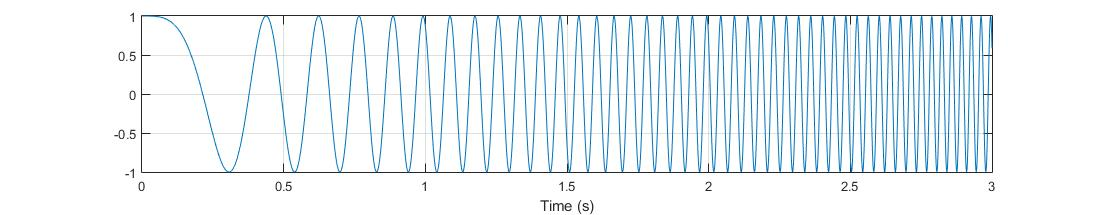
\includegraphics[width=1.1\textwidth]{Figuras/A.FrequencyResponseTest/A-ChirpSignal.jpg}}
	\caption{Chirp Signal}
	\label{fig:A_ChirpSignal}
\end{figure}

To obtain the system frequency response, the chirp input and the surface position output must be recorded. Then, the frequency response is obtained through manipulation of these signals.

According to \cite{IdtToolbox}, ``if the data is given in the time domain [$u(t)$ and $y(t)$], it is first converted to the frequency domain. Then averages of $Y(w)Conj(U(w))$ and $U(w)Conj(U(w))$ are formed over the frequency ranges $w$, corresponding to the desired resolution around the frequency in question. The ratio of these averages is then formed for the frequency-function estimate".

A flowchart for a test using a chirp input is shown in Figure \ref{fig:a4_3_2_1_ChirpFrequencyResponseFlowchart}.

\begin{figure}[H]
	\centering
	\centerline{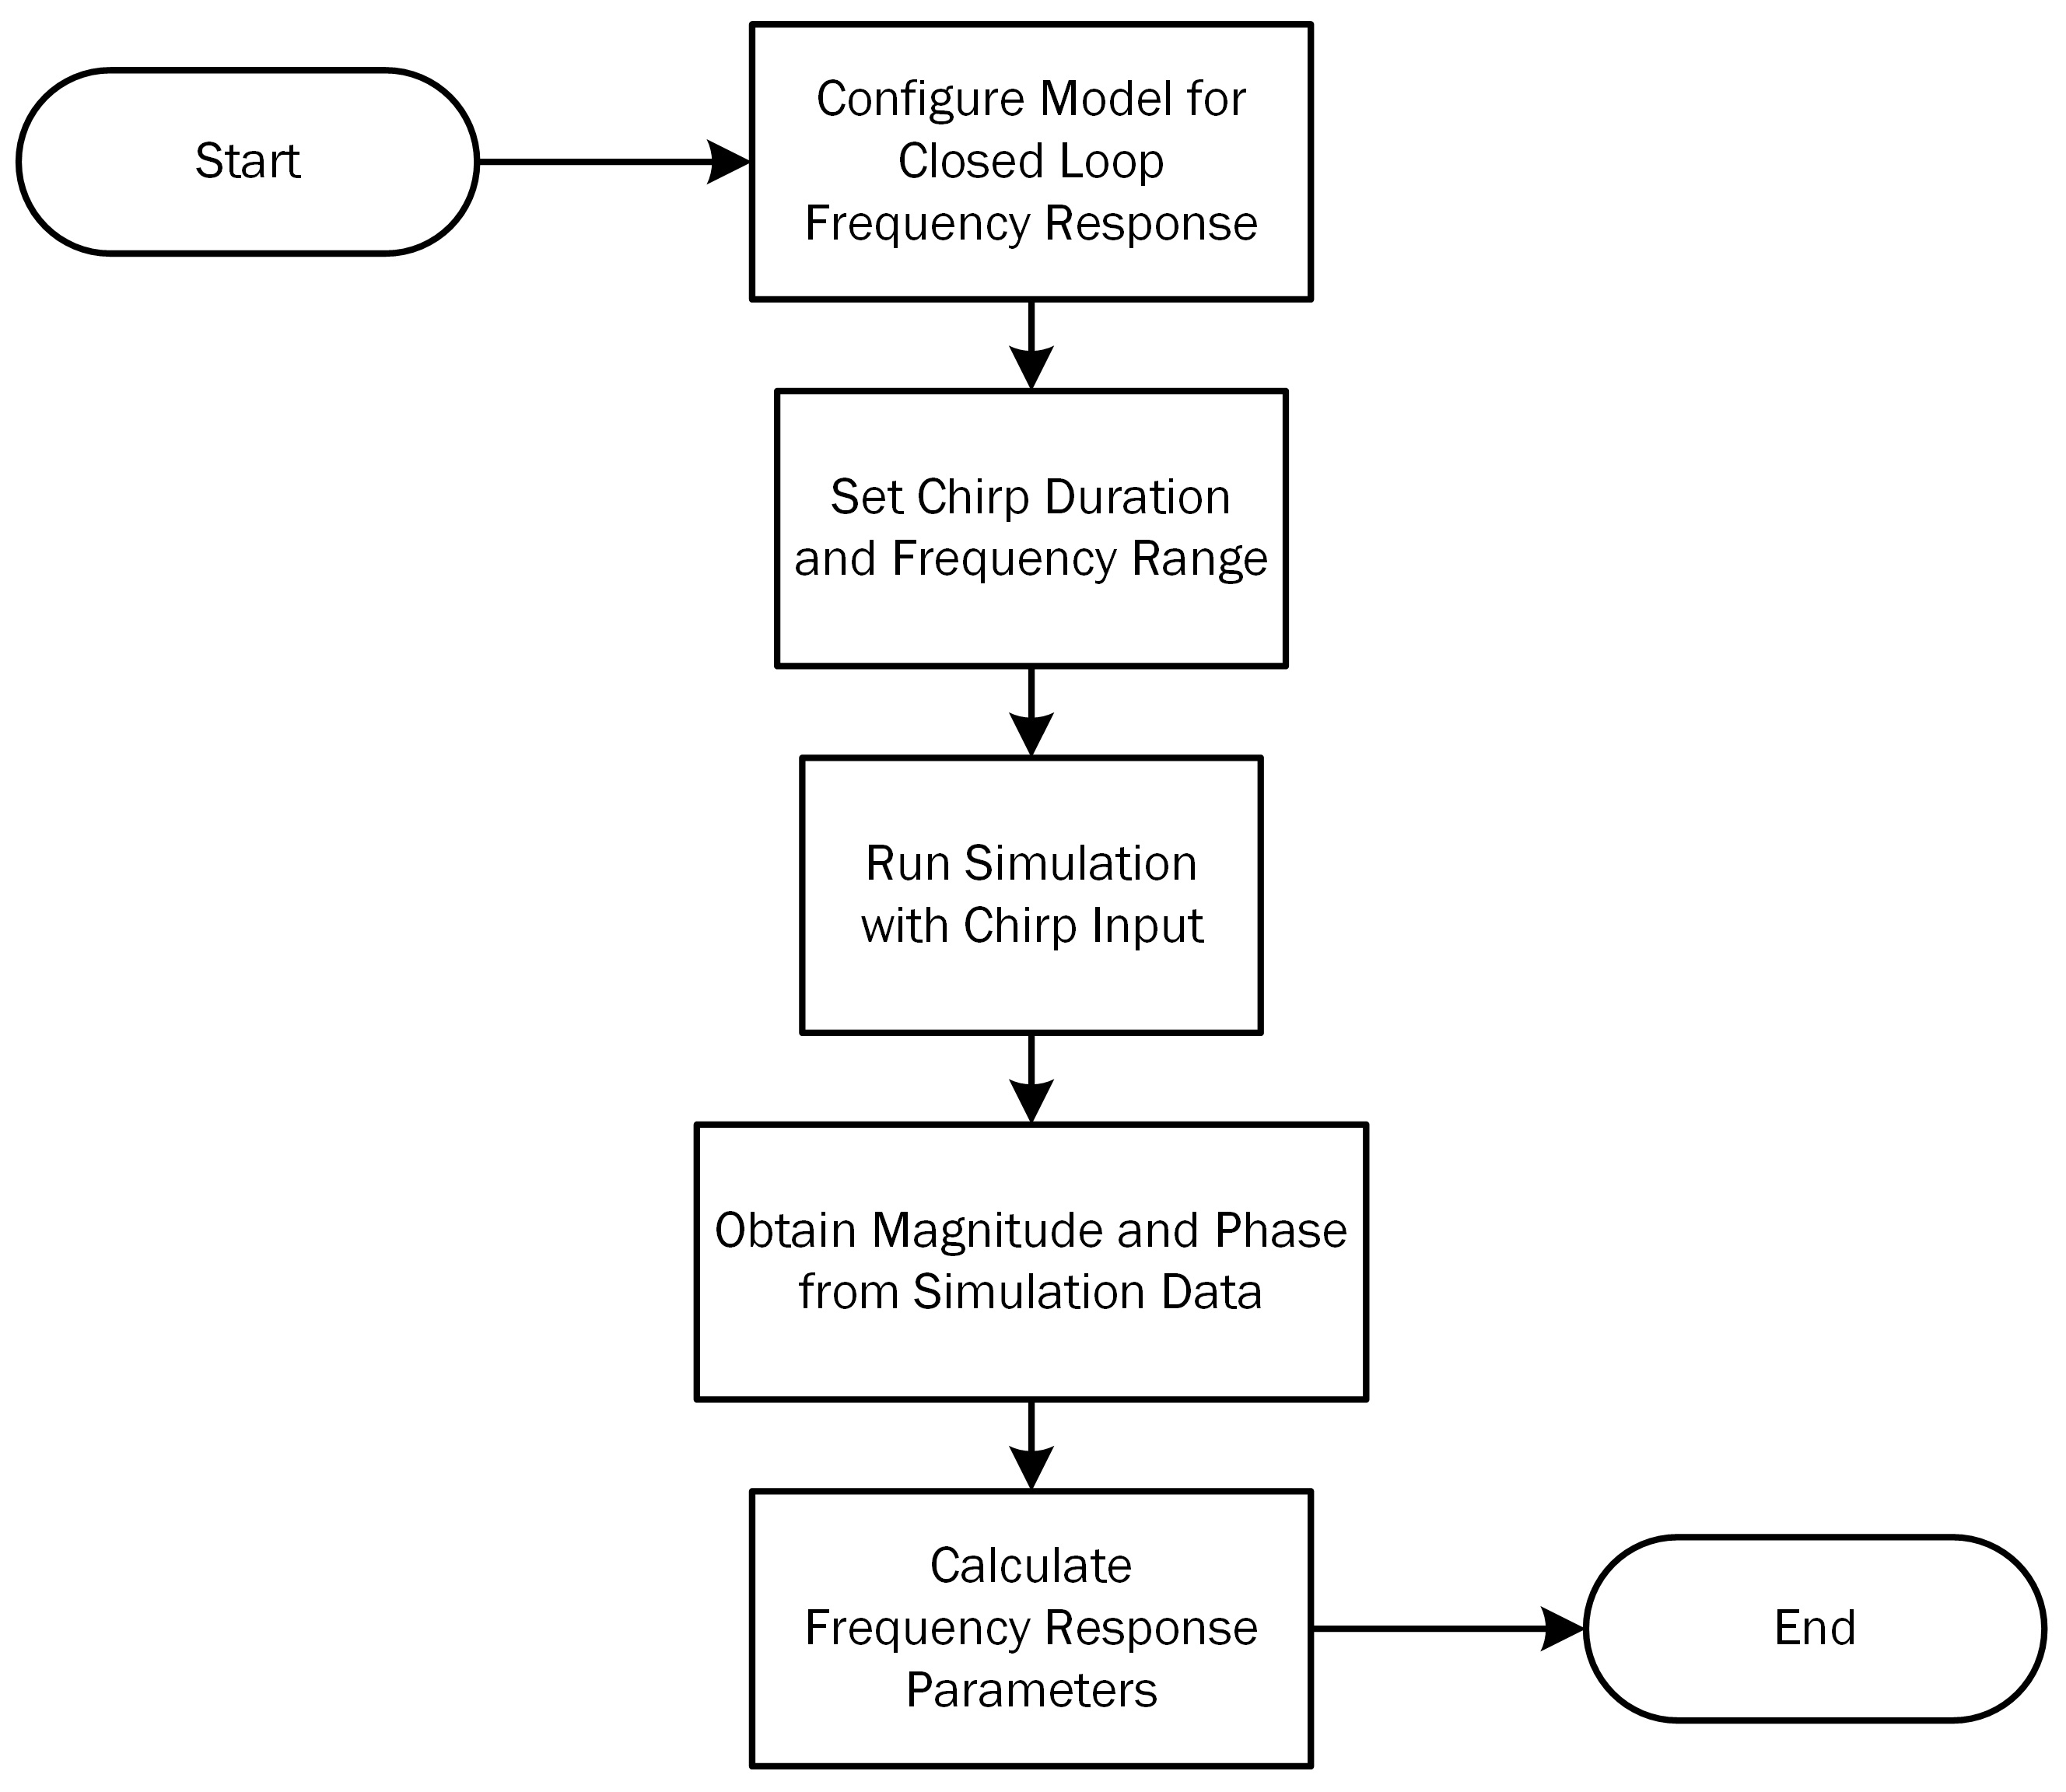
\includegraphics[width=0.7\textwidth]{Figuras/4.DynamicStifinessOptimizationAlgorithm/4-3-2-1-ChirpFrequencyResponse.jpg}}
	\caption{Flowchart of Frequency Response Test with Chirp Signal}
	\label{fig:a4_3_2_1_ChirpFrequencyResponseFlowchart}
\end{figure}

The first step, model configuration, is the same performed in the baseline test. Then, the following step is to customize the chirp input with its initial and final frequency as well as its length. The chirp frequencies were selected to match those evaluated by the baseline test and the chirp length was tested with three different values, as shown in Table \ref{table:A_ChirpScripParam}. 

\begin{table}[H]
	\captionof{table}{Chirp Frequency Response Test Parameters}
	\label{table:A_ChirpScripParam}
	\centering
	\resizebox{8cm}{!}{
		\begin{tabular}{|l|c|c|c|c|}
			\hline
			Parameter 					 & Value			\\ \hline
			Chirp Initial Frequency (Hz) & $0.1$				\\ \hline
			Chirp Final Frequency (Hz)	 & $35$			\\ \hline
			Chirp Signal Length (s)		 & $20$, $80$ and $100$	\\ \hline
	\end{tabular}}
\end{table}

After that, the simulation is executed and the results stored. The next step is to obtain magnitude and phase from the simulation data, what was evaluated with the MATLAB function \textit{spafdr}. This function manipulates data stored after simulation to produce a frequency-response model that can be used to obtain magnitude and phase information, as mentioned. The last step, the same for the baseline test, is to calculate the frequency constraint parameters.

Figure \ref{fig:A_ChirpScripResults} shows a comparison between magnitude and phase obtained with this test for different chirp signal lengths and the results obtained with baseline test.

\begin{figure}[H]
	\centering
	\centerline{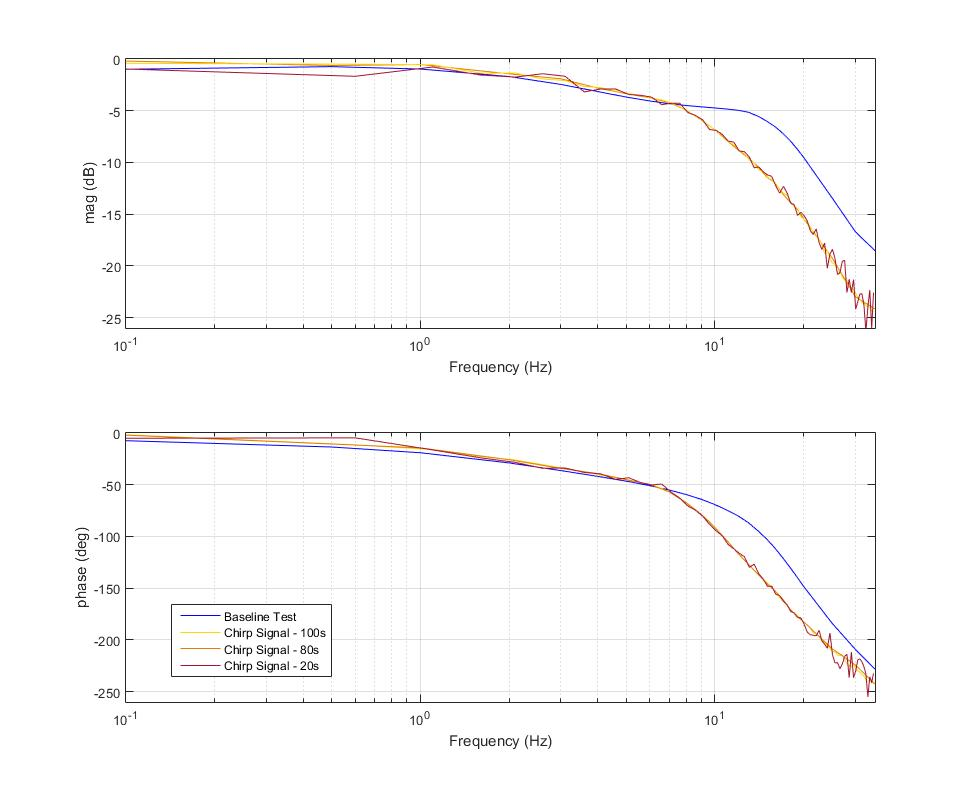
\includegraphics[width=0.9\textwidth]{Figuras/4.DynamicStifinessOptimizationAlgorithm/4-3-2-1-ChirpScripResults.jpg}}
	\caption{Baseline and Chirp Frequency Response Test Results Comparison}
	\label{fig:A_ChirpScripResults}
\end{figure}

The figure shows that for frequencies above 7 Hz the frequency responses given by \textit{spafdr} diverge from the baseline response, independently of the chirp signal length. This discrepancy has been attributed to model non-linearities that are not sufficiently captured either by the chirp signal itself or the \textit{spafdr} algorithm. 

Table \ref{table:A_ChirpScripResults} presents a performance comparison between the different input durations. The execution time for 80 and 100 seconds chirp signals is approximately 5 times the time to execute the baseline frequency response which is not desired. On the other hand, the 20 seconds chirp input is executed in 2.3 minutes, 82\% less time than the baseline response, which is a remarkable improvement in performance.

\begin{table}[H]
	\captionof{table}{Baseline and Chirp Frequency Response Test Comparison}
	\label{table:A_ChirpScripResults}
	\centering
	\resizebox{9cm}{!}{
		\begin{tabular}{|l|c|c|c|c|}
			\hline
			Constraint 							& Baseline	& \multicolumn{3}{|c|}{Chirp}  	\\ \hline
			Chirp Signal Length (s) 			& -			& $100$	 & $80$	  & $20$		\\ \hline
			Closed-Loop Gain Allowance (dB) 	& $13.0$	& $15.2$ & $15.0$ & $14.7$	 	\\ \hline
			Closed-Loop Phase Allowance ($°$)	& $Inf$  	& $Inf$	 & $Inf$  & $Inf$		\\ \hline
			Closed-Loop Bandwidth (Hz) 			& $5.8$  	& $5.3$	 & $4.7$  & $6.6$		\\ \hline
			Execution Time (min)				& $12.6$	& $60$	 & $55$   &	$2.3$		\\ \hline
	\end{tabular}}
\end{table}

Even though the execution time was reduced by 82\%, the chirp input test was discarded since its result does not match the baseline test.

\section{ARX Identification Frequency Response Test}

Another alternative method considered was to use model identification techniques to find an equivalent non-linear model and then use the baseline test to obtain the frequency response of this model. 

This strategy differs from the one presented previously because, instead of reducing the number of simulations, it adds one simulation and a model identification process. 

Despite this, the simulations performed by the baseline test on the identified model will be faster since the simulated model will be significantly simpler. Figure \ref{fig:a4_3_2_2_ARXFrequencyResponseFlowchart} shows the flowchart of this approach.

\begin{figure}[H]
	\centering
	\centerline{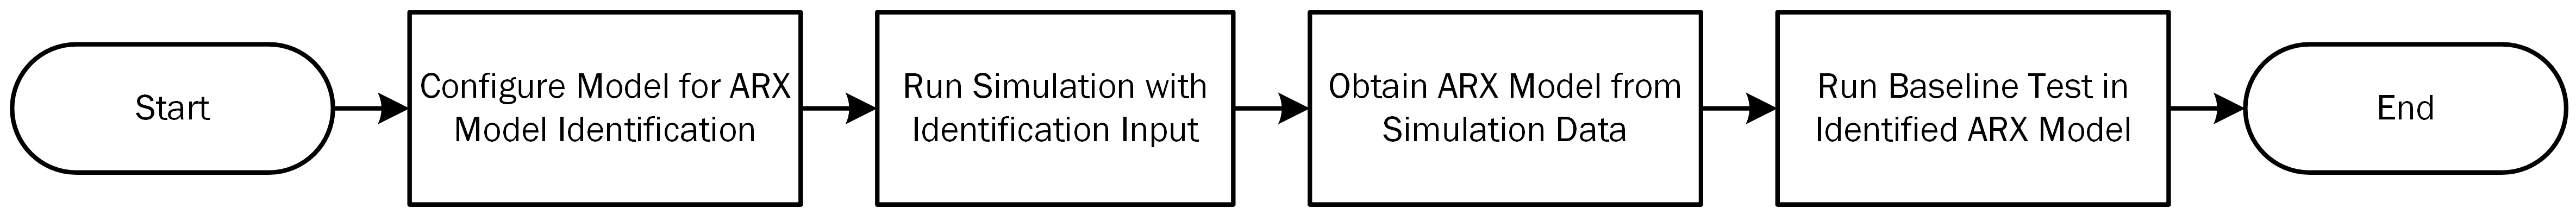
\includegraphics[width=0.9\textwidth]{Figuras/A.FrequencyResponseTest/A-ARXFrequencyResponse.jpg}}
	\caption{Flowchart of Frequency Response Test with ARX Identification}
	\label{fig:a4_3_2_2_ARXFrequencyResponseFlowchart}
\end{figure}

The first step is to configure the model to receive an identification signal (Figure \ref{fig:A_IdentificationSignalInput}) as input. Then, the model is simulated and data is generated for the identification process. 

\begin{figure}[H]
	\centering
	\centerline{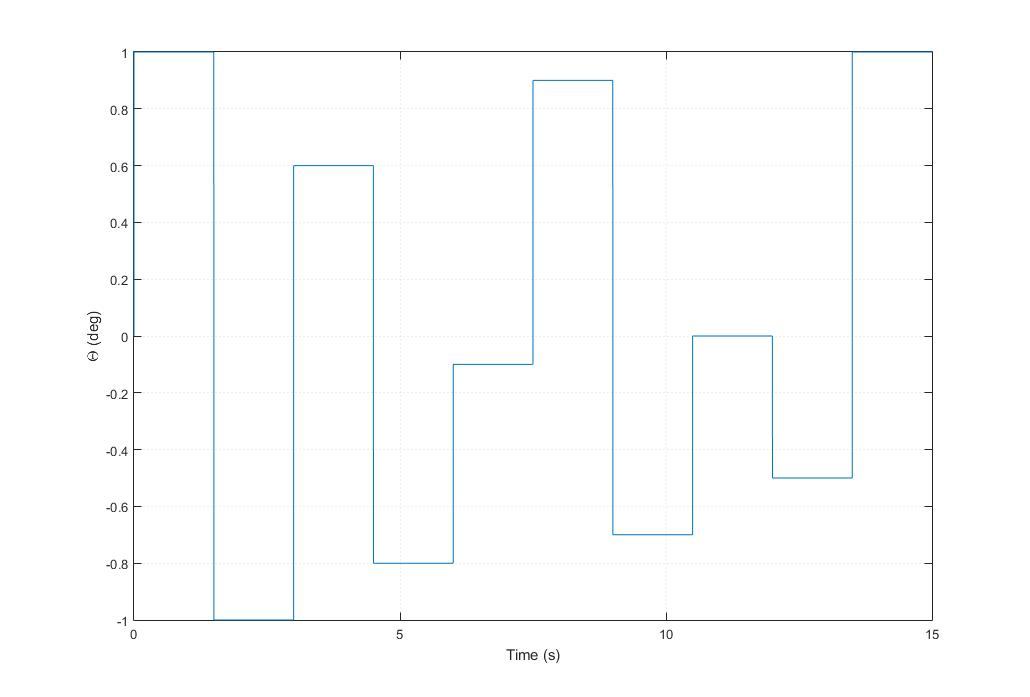
\includegraphics[width=0.9\textwidth]{Figuras/A.FrequencyResponseTest/A-IdentificationInput.jpg}}
	\caption{Identification Signal}
	\label{fig:A_IdentificationSignalInput}
\end{figure}

Next, the ARX model is obtained using \textit{nlarx}. Three types of nonlinearity estimators were used to evaluate this strategy: \textit{wavenet}, \textit{sigmoidnet} and \textit{treepartition}. Default configurations of these estimators were used but several model orders were evaluated for each nonlinearity estimator. 

\begin{figure}[H]
	\centering
	\centerline{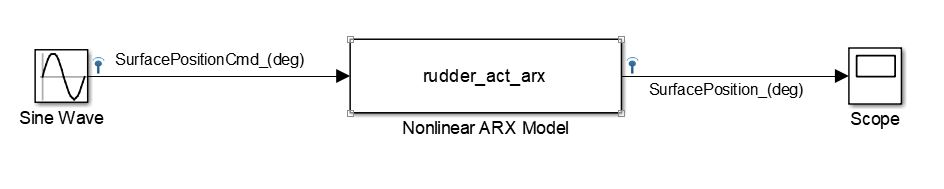
\includegraphics[width=0.9\textwidth]{Figuras/A.FrequencyResponseTest/A-SimplifiedModel.jpg}}
	\caption{Simulink Model for Baseline Frequency Response Test}
	\label{fig:A_SimplifiedModel}
\end{figure}

After obtaining the ARX model, the baseline frequency response test is performed in the simplified system model shown in Figure \ref{fig:A_SimplifiedModel}. 

Figure \ref{fig:A_ARXScripResults} shows the obtained responses for the model orders that responded most closely to the baseline test response.

\begin{figure}[H]
	\centering
	\centerline{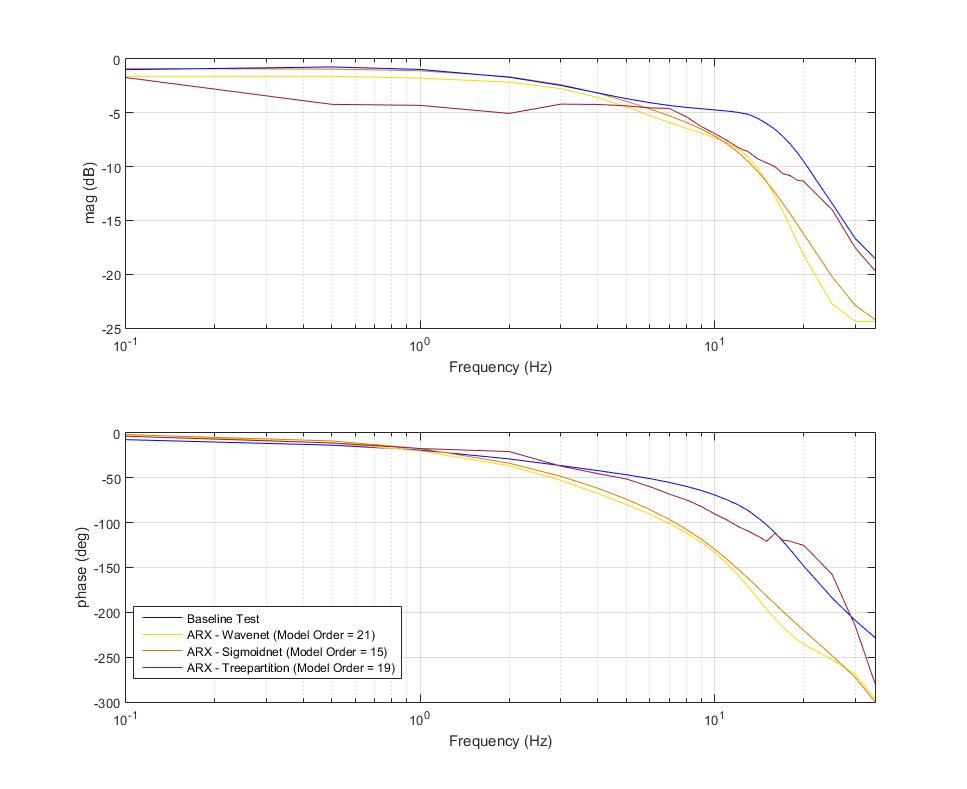
\includegraphics[width=0.9\textwidth]{Figuras/A.FrequencyResponseTest/A-ARXScriptResults.jpg}}
	\caption{Baseline and ARX Model Identification Frequency Response Test Results Comparison}
	\label{fig:A_ARXScripResults}
\end{figure}

Figure \ref{fig:A_ARXScripResults} shows that with estimators \textit{wavenet} and \textit{sigmoidnet} the magnitude frequency response of the identified ARX model matched the baseline test for frequencies up to 5Hz. However, above 5Hz, these responses diverged from the expected and behaved similarly to the chirp test response. The result obtained with the \textit{treepartition} ARX model matched the baseline test only for frequencies around 7Hz and 30Hz. The phase responses matched the expected only until 1Hz, after that results for all estimators diverged.

\begin{table}[H]
	\captionof{table}{Baseline and ARX Model Identification Frequency Response Test Results Comparison}
	\label{table:A_ARXScripResults}
	\centering
	\resizebox{12cm}{!}{
		\begin{tabular}{|l|c|c|c|c|}
			\hline
			Constraint 							& Baseline	& \multicolumn{3}{|c|}{ARX Model}  		\\ \hline
			Nonlinearity estimator				& -			& wavenet & sigmoidnet & treepartition	\\ \hline
			Closed-Loop Gain Allowance (dB) 	& $13.0$	& $9.8$	  & $11.2$	   & $15.4$	 		\\ \hline
			Closed-Loop Phase Allowance ($°$)	& $Inf$  	& $Inf$	  & $Inf$  	   & $Inf$			\\ \hline
			Closed-Loop Bandwidth (Hz) 			& $5.8$  	& $5.2$	  & $5.0$  	   & $1.6$			\\ \hline
			Execution Time (min)				& $12.6$	& $1.66$  & $1.95$ 	   & $5.15$			\\ \hline
	\end{tabular}}
\end{table}

Table \ref{table:A_ARXScripResults} presents the performance comparison between the baseline test and the ARX model for each estimator. Despite the significant execution time reduction, up to 87\%, the responses for these alternatives did not match closed-loop gain allowance and bandwidth at all. Therefore, this alternative was also discarded.

\section{Linear Model Frequency Response Test}

The next alternative evaluated was to use the baseline test to obtain the frequency response of a linearized model of the actuation system. This strategy was assessed with the linearization presented by Ballesteros (2015):

\begin{scriptsize}
	\begin{center}
		$\begin{bmatrix}
		\dot{x_v} \\
		\ddot{x_v} \\
		\dddot{x_v} \\
		\dot{\Delta P} \\
		\dot{x_p} \\
		\ddot{x_p} \\
		\end{bmatrix} =\begin{bmatrix}
		0 & 1 & 0 & 0 & 0 & 0\\
		0 & 0 & 1 & 0 & 0 & 0\\
		-1.77 \cdot 10^{10} & -2.11 \cdot 10^7 & -3.64 \cdot 10^3 & 0 & 0 & 0\\
		2.30 \cdot 10^7  & 0 & 0 & -9.36 \cdot 10^{-2} & 8.16 \cdot 10^1 & -9.63 \cdot 10^4\\
		0 & 0 & 0 & 0 & 0 & 1\\
		0 & 0 & 0 & 2.18 & 0 & -4.67 \cdot 10^1 \\
		\end{bmatrix}
		\begin{bmatrix}
		x_v \\
		\dot{x_v} \\
		\ddot{x_v} \\
		\Delta P \\
		x_p \\
		\dot{x_p} \\
		\end{bmatrix}
		+
		\begin{bmatrix}
		0 \\
		0 \\
		3.28 \cdot 10^7 \\
		0 \\
		0 \\
		0 \\
		\end{bmatrix}
		i
		$
	\end{center}
\end{scriptsize}
\begin{footnotesize}
	\begin{center}
		$\begin{bmatrix}
		x_v \\
		\Delta P \\
		x_p \\
		\end{bmatrix} =
		\begin{bmatrix}
		1 & 0 & 0 & 0 & 0 & 0\\
		0 & 0 & 0 & 1 & 0 & 0\\
		0 & 0 & 0 & 0 & 1 & 0\\
		\end{bmatrix}
		\begin{bmatrix}
		x_v \\
		\dot{x_v} \\
		\ddot{x_v} \\
		\Delta P \\
		x_p \\
		\dot{x_p} \\
		\end{bmatrix} $
	\end{center}
\end{footnotesize}

A comparison between the baseline strategy and this alternative is presented in Figure \ref{fig:A_LinearBaselineScriptResults}.

\begin{figure}[H]
	\centering
	\centerline{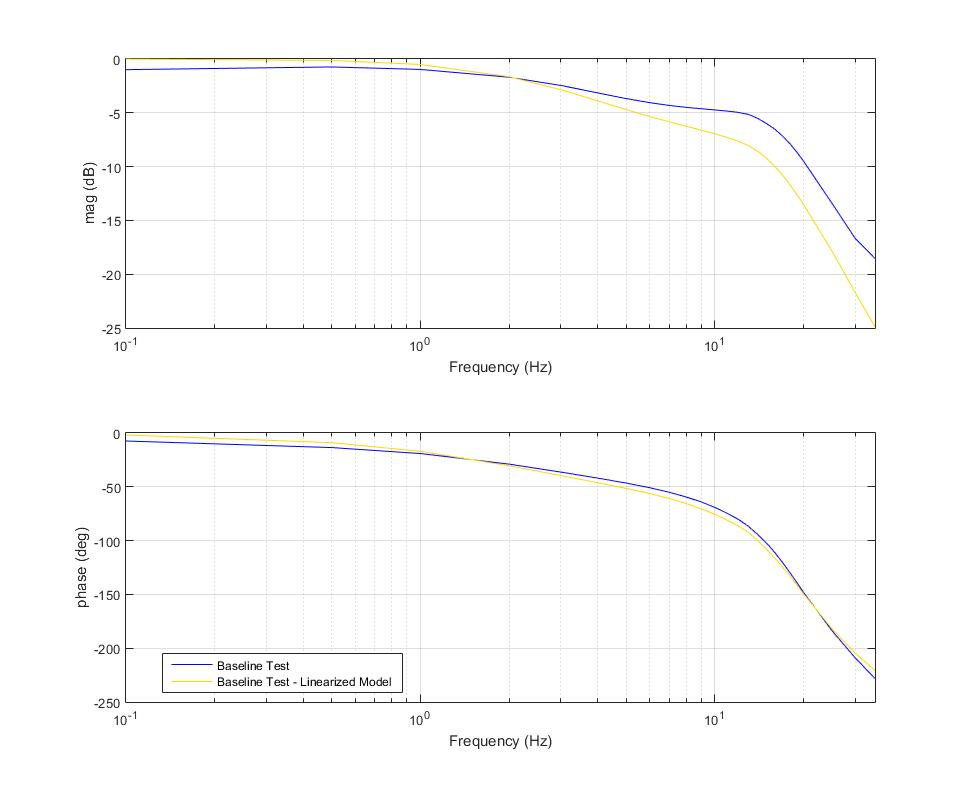
\includegraphics[width=0.9\textwidth]{Figuras/4.DynamicStifinessOptimizationAlgorithm/4-3-2-3-LinearBaselineScriptResults.jpg}}
	\caption{Non-Linear and Linearized Model Frequency Response Test Results Comparison}
	\label{fig:A_LinearBaselineScriptResults}
\end{figure}

Figure \ref{fig:A_LinearBaselineScriptResults} shows that the frequency response of the linearized model does not match the non-linear model response, specially in magnitude. This indicates that even for small inputs, of 0.5 degrees, the linear model is not able to replicate the non-linear model frequency response. 

Further investigation showed that for a 0.5 degree sine amplitude the EHSV current reached almost 4mA. These value is distant from the point where the system was linearized (0mA). EHSV current step input simulations were performed and confirmed that some dynamics of the model are not well represented in the linear model for this current. 

Table \ref{table:A_LinearBaselineScriptResults} shows the impact of this behavior in closed-loop gain allowance and bandwidth of the linearized model that were fairly different from the ones obtained by the baseline test. Despite this, the execution time of this alternative was approximately 60\% lower than the baseline, as expected.

\begin{table}[H]
	\captionof{table}{Non-Linear and Linearized Model Frequency Response Comparison}
	\label{table:A_LinearBaselineScriptResults}
	\centering
	\resizebox{8cm}{!}{
		\begin{tabular}{|l|c|c|c|c|}
			\hline
			Constraint 				& Baseline 	& Linearized Model	\\ \hline
			Closed-Loop Gain Allowance (dB) 		& $13.0$	& $17.6$			\\ \hline
			Closed-Loop Phase Allowance ($°$)		& $Inf$  	& $Inf$	  			\\ \hline
			Bandwidth (Hz) 			& $5.8$  	& $3.1$				\\ \hline
			Execution Time (min)	& $12.6$	& $4.28$			\\ \hline
	\end{tabular}}
\end{table}

At this point, it was clear that finding alternative methods that could both save execution time and replicate the baseline's response was very challenging. The next step then was in the direction to improve the baseline test's execution time, rather than to find an alternative strategy.

\section{Modified Baseline Frequency Response Test}

Since the execution time of the baseline test is mostly the time to execute all simulations, their duration was revisited. Instead of calculating simulation's length only from input signal cycles, a non variable time parameter was introduced with the aim to capture model dynamics settling time. The duration of each simulation was calculated with Equation \ref{eq:A_SimulationDuration}.

\begin{equation}
\label{eq:A_SimulationDuration}
T\textsubscript{sim} = T\textsubscript{dyn} + K\textsubscript{int} \times T_p
\end{equation}

T\textsubscript{sim} is the simulation duration for each frequency whereas T\textsubscript{dyn} is the model dynamics settling time. This constant parameter was obtained empirically from measuring the amplitude of actuator surface position in simulations with sine input for several frequencies which yielded a 0.5 seconds settling time.

Parameter $K\textsubscript{int}$ is the number of integration cycles for the respective frequency and $T_p$ is the frequency's period. $K\textsubscript{int}$ was selected to minimize simulation time but in a way that did not jeopardize the frequency response. Frequencies 0.1, 0.5 and 1 Hz were integrated for only one cycle while three cycles were considered for 2 and 3 Hz and nine cycles for frequencies from 4 to 35 Hz. A comparison between the baseline and modified tests is presented in Figure \ref{fig:A_ModifiedBaselineScriptResults}.

The figure shows that magnitude and phase responses for both tests match in most frequencies. Even though there is a difference between the curves at around 13 Hz, the overall response of the modified test is suitable for constraint evaluation purposes. It is important to remark that the baseline test will be used to evaluate initial and optimized controllers prior and after optimization.

\begin{figure}[H]
	\centering
	\centerline{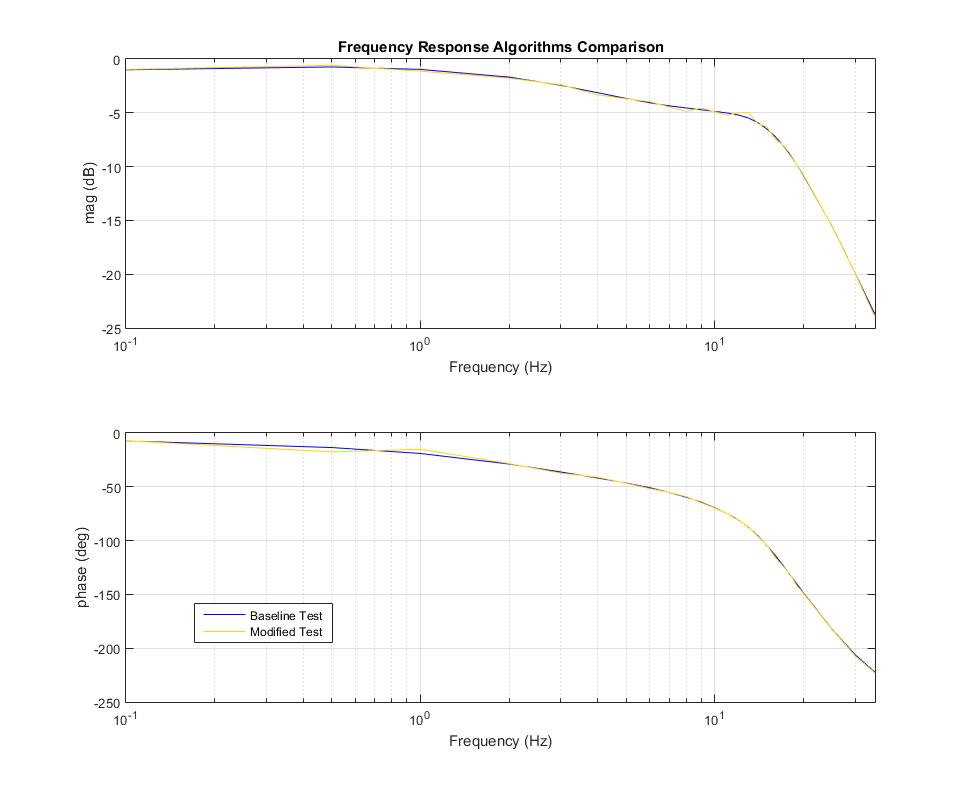
\includegraphics[width=0.9\textwidth]{Figuras/4.DynamicStifinessOptimizationAlgorithm/4-3-2-4-ModifiedBaselineScriptResults.jpg}}
	\caption{Baseline and Modified Frequency Response Test Results Comparison}
	\label{fig:A_ModifiedBaselineScriptResults}
\end{figure}

Table \ref{table:A_ModifiedBaselineScriptResults} shows the closed-loop gain and phase allowances for both tests are the same and that bandwidth slightly increases. Also, execution time reduced considerably, falling from 12.6 to 4.85 minutes.

\begin{table}[H]
	\captionof{table}{Baseline and Modified Frequency Response Test Results Comparison}
	\label{table:A_ModifiedBaselineScriptResults}
	\centering
	\resizebox{8cm}{!}{
		\begin{tabular}{|l|c|c|c|c|}
			\hline
			Constraint 				& Baseline 	& Modified 			\\ \hline
			Closed-Loop Gain Allowance (dB) 		& $13.0$	& $13.0$			\\ \hline
			Closed-Loop Phase Allowance ($°$)		& $Inf$  	& $Inf$	  			\\ \hline
			Bandwidth (Hz) 			& $5.8$  	& $6.0$				\\ \hline
			Execution Time (min)	& $12.6$	& $4.85$			\\ \hline
	\end{tabular}}
\end{table}

The modified test is executed in approximately 60\% less time than the baseline. Table \ref{table:A_ModifiedBaselineScriptTimeComparison} presents an execution time breakdown for both tests and the difference between them.

Simulations in lower frequencies have the longest durations due to their large periods, even though they have few integration cycles. Despite this, time savings were observed in all simulations and most of them were reduced by more than 50\%.

\begin{table}[H]
	\captionof{table}{Baseline and Modified Frequency Response Test Execution Time Comparison}
	\label{table:A_ModifiedBaselineScriptTimeComparison}
	\centering
	\resizebox{15cm}{!}{
		\begin{tabular}{|c|c|c|c|c|}
			\hline
			Frequency (Hz) & Baseline Exec. Time (s) & Modified Exec. Time (s) & Time Reduction (s) & Percentual Red. (\%) \\ \hline
			0.1			   & 171  & 59.8 & -111  & -65.1 \\ \hline
			0.5			   & 36.0 & 15.3 & -20.7 & -57.5 \\ \hline
			1			   & 18.9 & 9.76 & -9.10 & -48.3 \\ \hline
			2			   & 20.3 & 12.5 & -7.86 & -38.7 \\ \hline
			3			   & 18.6 & 9.71 & -8.84 & -47.7 \\ \hline
			4			   & 18.3 & 13.7 & -4.59 & -25.1 \\ \hline
			5			   & 18.2 & 11.9 & -6.29 & -34.6 \\ \hline
			6			   & 18.7 & 10.6 & -8.11 & -43.4 \\ \hline
			7			   & 18.6 & 9.70 & -8.90 & -47.9 \\ \hline
			8			   & 20.8 & 9.01 & -11.8 & -56.6 \\ \hline
			9			   & 18.1 & 8.49 & -9.59 & -53.0 \\ \hline
			10			   & 18.0 & 8.03 & -9.97 & -55.4 \\ \hline
			11			   & 18.1 & 7.75 & -10.3 & -57.1 \\ \hline
			12			   & 18.1 & 7.45 & -10.7 & -58.9 \\ \hline
			13			   & 18.2 & 7.11 & -11.1 & -61.0 \\ \hline
			14			   & 18.3 & 7.09 & -11.2 & -61.2 \\ \hline
			15			   & 18.0 & 6.68 & -11.3 & -62.8 \\ \hline
			16			   & 18.2 & 6.52 & -11.7 & -64.1 \\ \hline
			17			   & 18.0 & 6.46 & -11.6 & -64.2 \\ \hline
			18			   & 18.6 & 6.38 & -12.2 & -65.7 \\ \hline
			19			   & 18.2 & 6.16 & -12.0 & -66.1 \\ \hline
			20			   & 18.0 & 6.08 & -11.9 & -66.2 \\ \hline
			25			   & 18.0 & 5.80 & -12.2 & -67.8 \\ \hline
			30			   & 18.0 & 5.44 & -12.6 & -69.8 \\ \hline
			35			   & 18.3 & 5.27 & -13.0 & -71.2 \\ \hline
			Total		   & 10.5 min & 4.38 min & -6.15 min & -58.4\% \\ \hline
	\end{tabular}}
\end{table}

In summary, several strategies to obtain the frequency response of the actuation system model were investigated and none of them were suitable to substitute the baseline test. Despite this, considerable execution time reductions were observed also in all strategies what indicates that it is still worth to study these strategies. 

Nevertheless, an alternative solution was adopted by reassessing the length of simulations in the baseline frequency response test. This alternative test was used solely to evaluate optimization constraints while the frequency performance of initial and optimized controllers was still evaluated with the baseline test.

%
%\section{Dynamic Stiffness Test} 
%
%The dynamic stiffness is obtained similarly to the frequency response, through simulation of the model for each evaluated frequency and further processing of the data generated by these simulations. Figure \ref{fig:a4_4_1_DynamicStiffnessTestFlowchart} shows the flowchart of this test.
%
%\begin{figure}[H]
%	\centering
%	\centerline{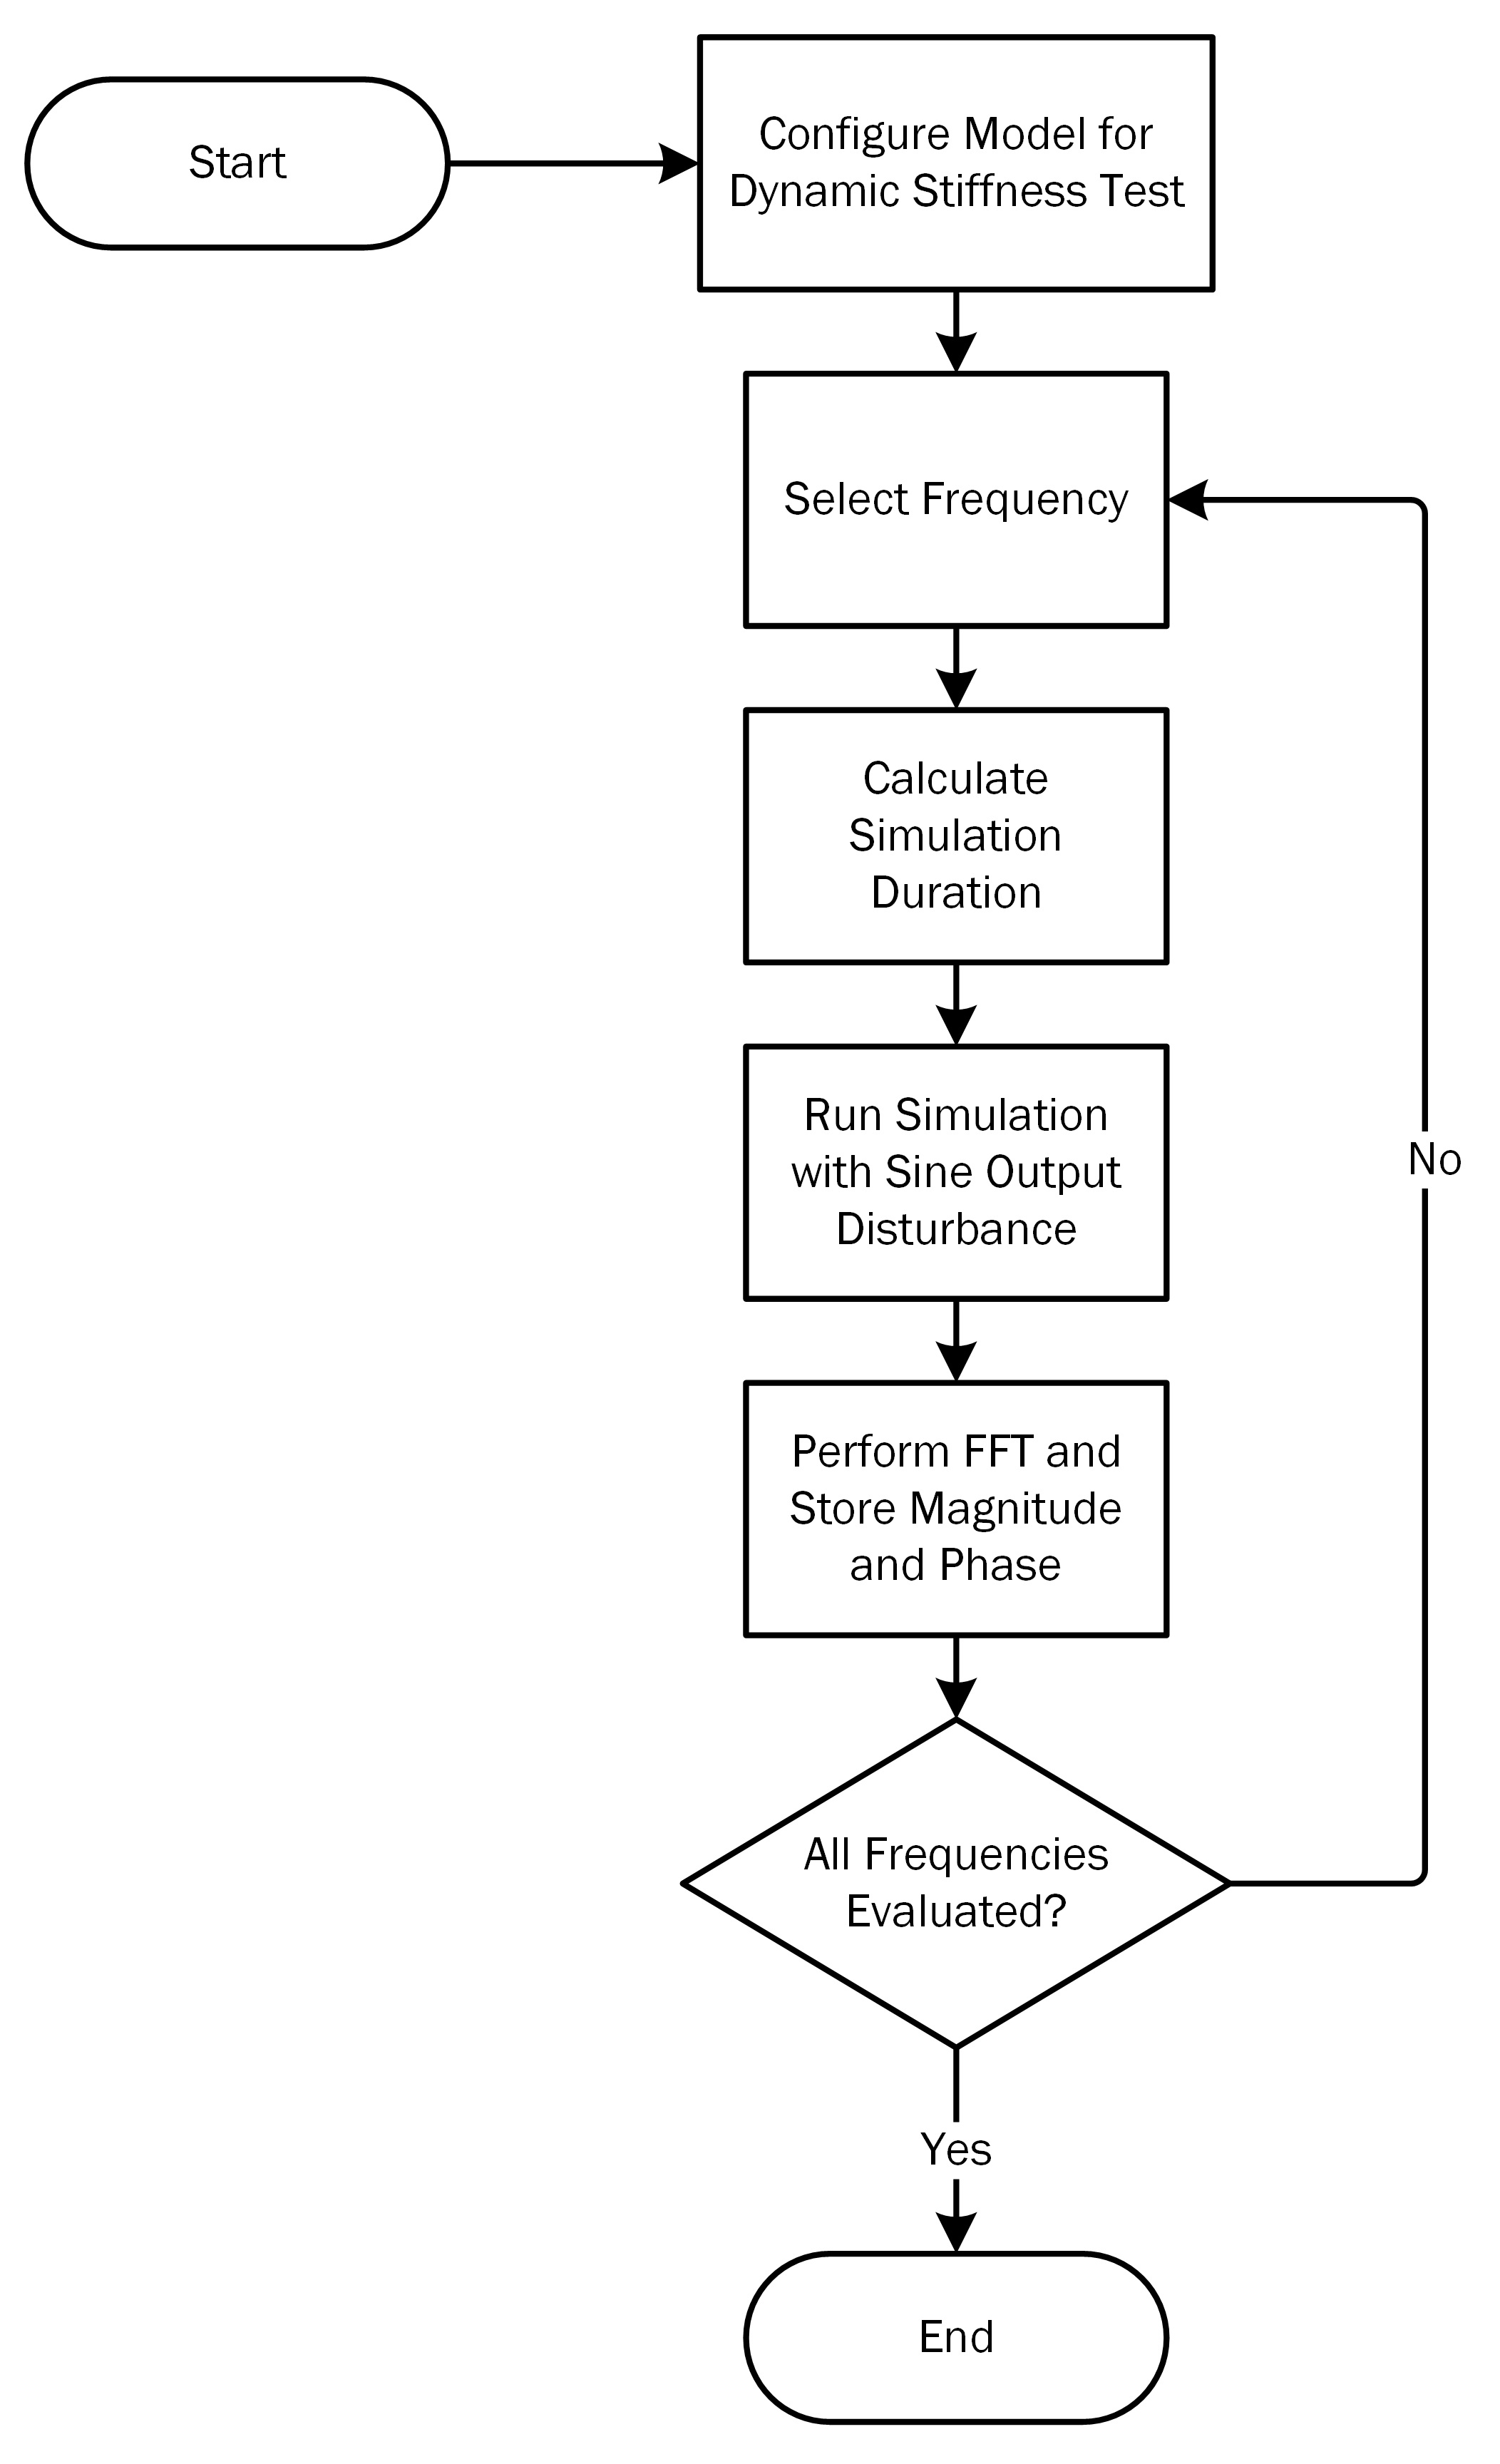
\includegraphics[width=0.6\textwidth]{Figuras/4.DynamicStifinessOptimizationAlgorithm/4-4-1-DynamicStiffnessTest.jpg}}
%	\caption{Dynamic Stiffness Test Flowchart}
%	\label{fig:a4_4_1_DynamicStiffnessTestFlowchart}
%\end{figure}
%
%First, the model is configured to the following test condition:
%
%\begin{enumerate}[a)]
%	\item Single actuator connected to rudder surface;	
%	\item Initial position = 0$°$;
%	\item Position command = 0$°$;
%	\item Sinusoidal aerodynamic load disturbance between 0.1 and 0.5 of actuator stall load;
%	\item Maximum hydraulic supply pressure of 3000 psi;
%	\item Maximum hydraulic return pressure of 150 psi;	
%	\item At 100$°C$ (212$°F$) fluid temperature;	
%\end{enumerate}
%
%The test is performed with the highest fluid temperature of the operational envelope because, since the bulk modulus decreases when temperature rises, the fluid compressibility increases and that leads to lower dynamic stiffness. Since there is no surface command,  the flow in the cylinder chamber is not substantial and therefore the fluid density does not have a major influence in the response. Therefore, it is more conservative to evaluate actuator dynamic stiffness at 100$°C$. This behaviour will be evident in chapter \ref{Optimization Results}.
%
%Next, the aerodynamic load disturbance frequency to be evaluated is selected and the simulation duration period is calculated with the same method used in the baseline frequency response test. For frequencies up to 1 Hz, the duration spans for 3 complete sine cycles and, for frequencies between 1 Hz and 35 Hz, the number of cycles covered by the simulation is 3 times the evaluated frequency.
%
%After that, the simulation is performed and the sinusoidal load disturbance and the ram position values are stored. This information is processed in the next step, when a Fast Fourier Transform (FFT) is performed for both signals. The transformed vectors are divided by each other and the real part of the resulting value at the excitation frequency yields the dynamic stiffness. The last steps are repeated until the dynamic stiffness is obtained for all fequencies of interest.
%
%The execution time of the presented dynamic stiffness test is approximately 10 minutes which is a considerable computational cost. However, because this test is similar to the frequency response test, it is possible to implement the same modifications of the frequency response test in the dynamic stiffness test. 
%
%Hence, the dynamic stiffness test was modified and the duration of each simulation is now calculated with equation \ref{eq:4_3_2_3_SimulationDuration}. In addition, the same values of $K\textsubscript{int}$ were used for the same frequencies. 
%
%A comparison between both tests is shown in Figure \ref{fig:a4_4_1_DynamicStiffnessComparison}. The yellow curve shows the dynamic stiffness obtained from the modified test which is fairly similar to the one from the original test, in blue. Given that, the modified test can be used to evaluate the dynamic stiffness during optimization in order to reduce execution time. Despite this, the original dynamic stiffness test is still employed to obtain this characteristic of the initial and final solutions of the optimization.
%
%\begin{figure}[H]
%	\centering
%	\centerline{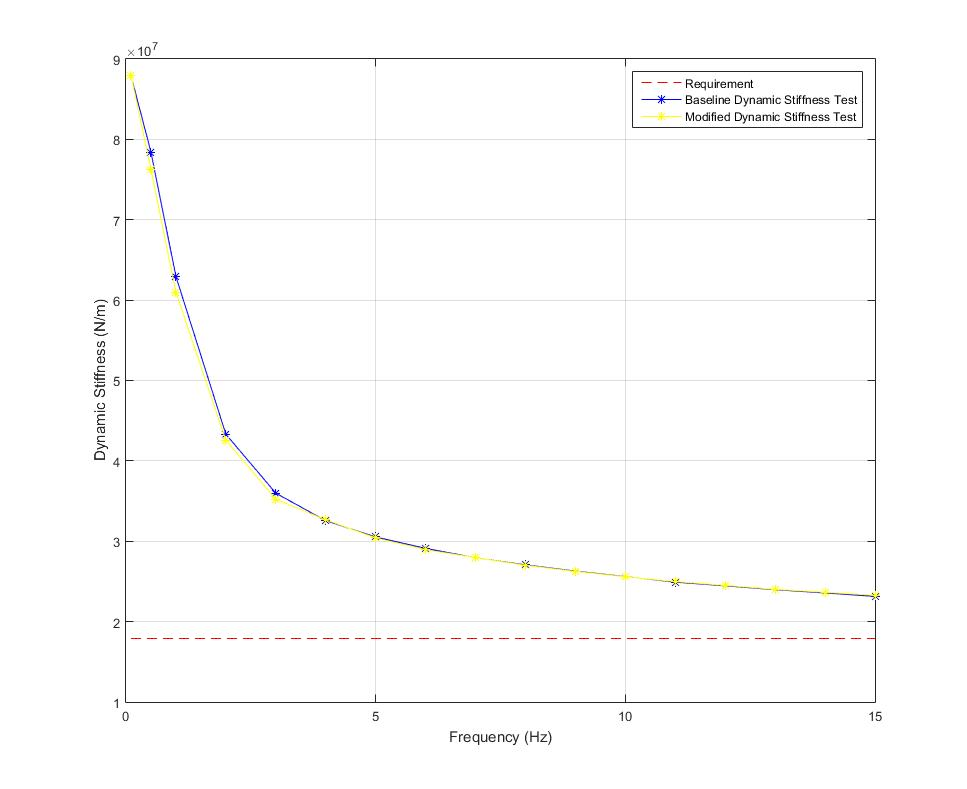
\includegraphics[width=0.9\textwidth]{Figuras/4.DynamicStifinessOptimizationAlgorithm/4-4-1-DynamicStiffnessComparison.jpg}}
%	\caption{Baseline and Modified Dynamic Stiffness Test Comparison}
%	\label{fig:a4_4_1_DynamicStiffnessComparison}
%\end{figure}
%
%The modified test is executed in approximately 43\% less time than the original test. Table \ref{table:a4_4_1_ModifiedDynStiffTestTimeComparison} presents an execution time breakdown for both tests and the difference between them.
%
%\begin{table}[H]
%	\captionof{table}{Baseline and Modified Dynamic Stiffness Test Execution Time Comparison}
%	\label{table:a4_4_1_ModifiedDynStiffTestTimeComparison}
%	\centering
%	\resizebox{12cm}{!}{
%		\begin{tabular}{|c|c|c|c|c|}
%			\hline
%			Frequency (Hz) & Baseline Exec. Time (s) & Modified Exec. Time (s) & Time Reduction (s) & Percentual Red. (\%) \\ \hline
%			0.1			   & 203  & 74.9 & -128  & -63.1 \\ \hline
%			0.5			   & 41.9 & 45.4 &  3.46 &  8.26 \\ \hline
%			1			   & 21.7 & 26.9 &  5.19 &  23.9 \\ \hline
%			2			   & 21.6 & 16.3 & -5.25 & -24.3 \\ \hline
%			3			   & 21.2 & 11.7 & -9.46 & -44.7 \\ \hline
%			4			   & 21.4 & 19.7 & -1.67 & -7.81 \\ \hline
%			5			   & 21.2 & 16.7 & -4.47 & -21.1 \\ \hline
%			6			   & 21.1 & 14.7 & -6.42 & -30.4 \\ \hline
%			7			   & 21.1 & 13.5 & -7.61 & -36.1 \\ \hline
%			8			   & 21.6 & 12.4 & -9.26 & -42.8 \\ \hline
%			9			   & 21.1 & 11.4 & -9.70 & -45.9 \\ \hline
%			10			   & 21.3 & 10.6 & -10.7 & -50.4 \\ \hline
%			11			   & 21.4 & 10.5 & -10.9 & -50.9 \\ \hline
%			12			   & 21.5 & 9.78 & -11.8 & -54.6 \\ \hline
%			13			   & 21.4 & 9.28 & -12.1 & -56.6 \\ \hline
%			14			   & 21.5 & 8.87 & -12.6 & -58.7 \\ \hline
%			15			   & 21.3 & 8.58 & -12.7 & -59.7 \\ \hline
%			Total		   & 9.42 min & 5.35 min & -4.07 min & -43.2\% \\ \hline
%	\end{tabular}}
%\end{table}
